\documentclass[12pt,twoside,onecolumn]{article}

\usepackage{a4}
\usepackage[dvipsnames]{xcolor}
\usepackage[margin=0.75in]{geometry}
\usepackage{pdfpages}
\usepackage{apacite}
\usepackage{jneurosci}
\usepackage[utf8]{inputenc}
\usepackage[T1]{fontenc}
\usepackage[norsk]{babel}
\usepackage{subfiles} % Handeling multiple chapters on seperate files.
\usepackage{graphicx}  % for displaying figures
\usepackage{subcaption}
\usepackage{url}
\usepackage{amsmath} % math package
\usepackage{relsize} % to use larger math symbols
\usepackage{amssymb} % for using blackboard letters (e.g R for real numbers)
\usepackage{tocbibind} % for adding the reference section in table of contents
%\usepackage{fixltx2e} % for text in sub script
\usepackage{perpage} % for resetting footnote counter at each page
\usepackage{csquotes}
\usepackage{epigraph}
\usepackage{ragged2e}
\usepackage{exercise}
\usepackage{amsmath}


\MakePerPage{footnote} %the perpage package command

\addto\captionsenglish{%
  \renewcommand{\figurename}{Figur}
}

\addto\captionsenglish{\renewcommand{\exercisename}{Oppgave}}

\makeatletter
\def\@documentnocite#1{\@bsphack
  \@for\@citeb:=#1\do{%
    \edef\@citeb{\expandafter\@firstofone\@citeb}%
    \if@filesw\immediate\write\@auxout{\string\citation{\@citeb}}\fi
    \@ifundefined{b@\@citeb}{\G@refundefinedtrue
      \@latex@warning{Citation `\@citeb' undefined}}{}}%
  \@esphack}
\AtBeginDocument{\let\nocite\@documentnocite}
\makeatother

\begin{document}

\hspace{-6mm}Denne skriften er det brukeren ser, inkludert skrift som er fargelagt {\color{red}rødt} og {\color{blue}blått}\newline
{\color{gray} Skriften brukes til å refere til manus} \newline
{\color{PineGreen} Skriften brukes til å refere til videodesigner} \newline
{\color{Maroon} Skriften brukes til å refere til handlinger i plattformen} \newline
{\color{Cerulean} Skriften brukes til å stille design spørsmål}

\section*{Ligninger}

\subsection*{Førstegradsligninger}

\begin{Exercise}
\begin{align}
7x - 3 &= 11  \qquad\text{ Plus 3 på begge sider av likhetstegnet.}\\
7x -3 +3 &= 11 + 3\\
7x &= 14\\  
\frac{7x}{7} &=  \frac{14}{7} \qquad\text{ Uttrykket kan forkenkles mer.}\\
x &= 2
\end{align}
\end{Exercise}

\begin{Exercise}
\textbf{Del 1}
\begin{align}
\frac{x}{2} + \frac{5}{6} &=  \frac{4}{3} - x \qquad\text{ Pluss x på begge sider av likhetstegnet.}\\
\frac{x}{2} + x + \frac{5}{6} &=  \frac{4}{3} - x + x\\
\frac{x}{2} + x + \frac{5}{6} - \frac{5}{6} &=  \frac{4}{3} - \frac{5}{6}\\
\frac{x}{2} + \frac{2x}{2} &= \frac{8}{6} - \frac{5}{6}\\
\frac{3x}{2}  &= \frac{3}{6} \qquad\text{ Uttrykket kan forkenkles mer.}\\ 
\frac{3x\cdot2}{7\cdot3} &=  \frac{1\cdot2}{2\cdot3} \qquad\text{ Uttrykket kan forkenkles mer.}\\
x &= \frac{1}{2}
\end{align}
\end{Exercise}

\subsection*{Sett inn tall i formler}
\begin{Exercise}
Fatima har kjøpt nytt abonnement hos Telihor. I abonnementet har hun en fast beløp hver måned på 50 kr. I tillegg må hun betale 1.50 kr per MB hun bruker. 
\newline\newline
\textbf{Del 1)} Lag en ligning som beskriver Fatimas total månedlig kostnad. La x være antall MB hun bruker i måneden og P(x) hennes total kostnad per måned.
\begin{align}
P &= 50 \text{ Hvis Fatima bruker ingen data, blir da hennes forbruk lik 50}\\ 
P &= 50 + 1.5\cdot1\text{ Hvis Fatima bruker 1MB data, blir da hennes forbruk lik $50 + 1.5\cdot1$}\\ 
P &= 50 + 1.5\cdot2\text{ Hvis Fatima bruker 2MB data, blir da hennes forbruk lik $50 + 1.5\cdot2$}\\ 
&\text{ Hva blir hennes forbruk hvis hun bruker x-antall data per måned} \nonumber\\
P &= 50 + 1.5x
\end{align}
\newline
\textbf{Del 2)}
Finn hennes total kostnad per måned når hun bruker 1000 MB = 1 GB data.
\begin{align}
P &= 50 + 1.5\cdot1000\\
P &= 50 + 1500\\
P &= 1550
\end{align}
Vil du si at dette er et bra abonnement for Fatima i år 2017 ?
\end{Exercise}

\section*{Funksjoner}

\begin{Exercise}
Vennligst klikk følgende koordinat i planet:$(0,1)$
\begin{figure}[h!]
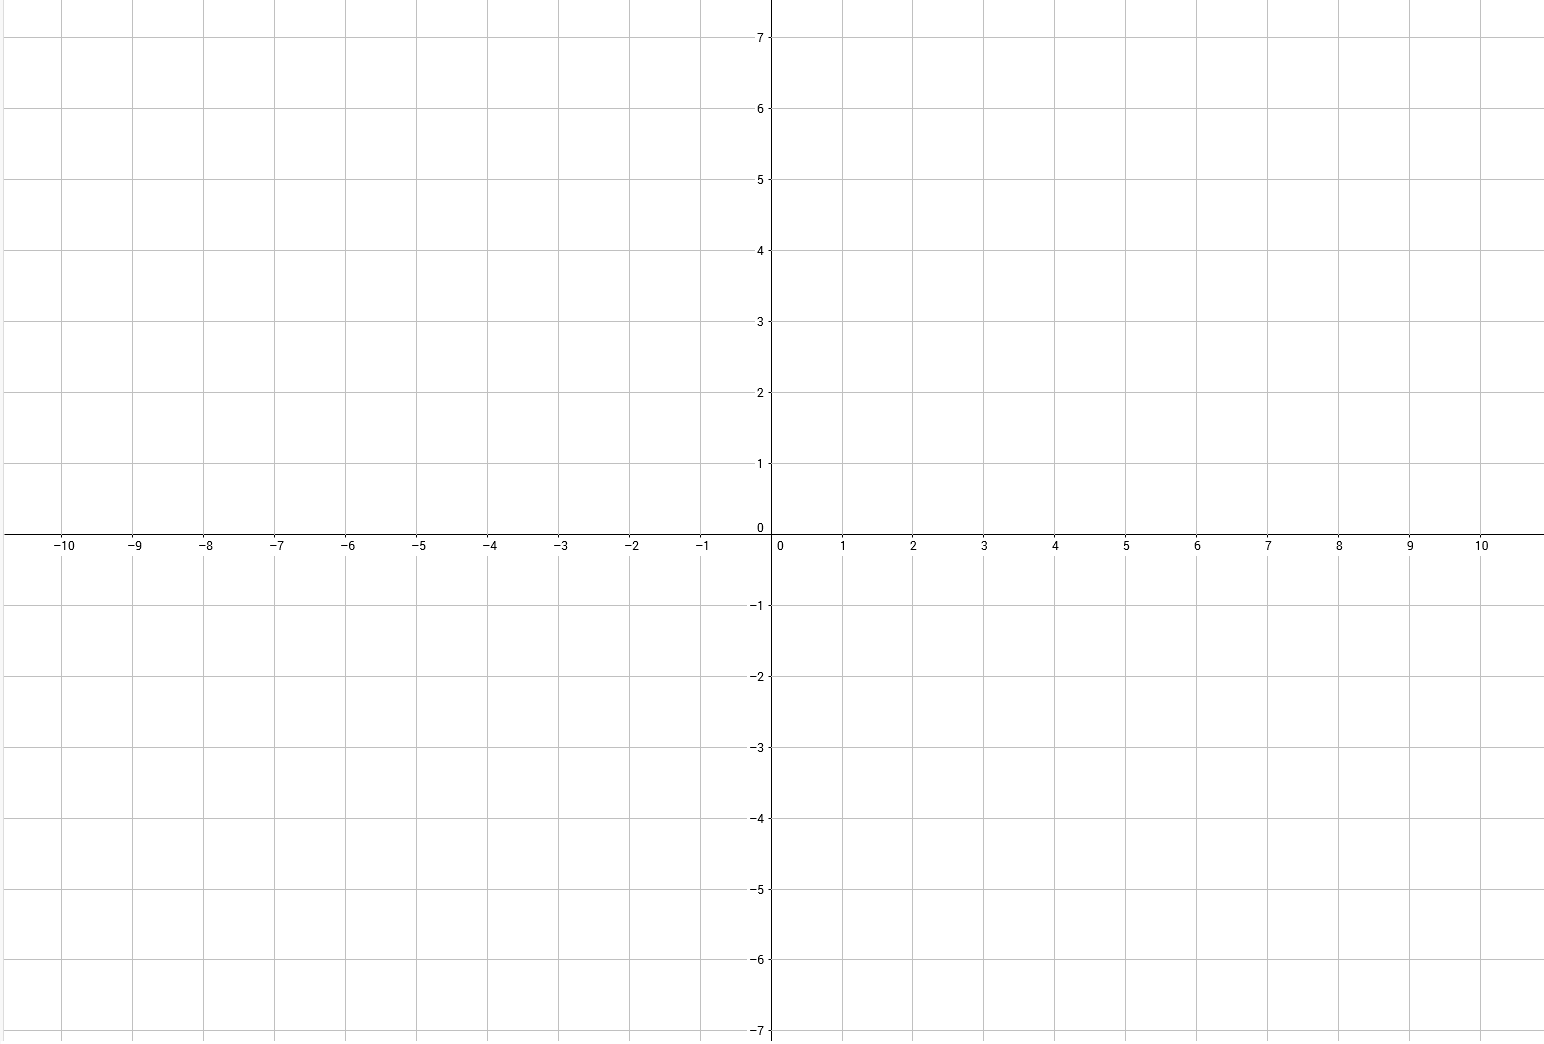
\includegraphics[scale = 0.3]{figures/Grid.png}
\label{fig:grid}
\end{figure}
\newline
{\color{Maroon}Hvis bruker taster feil, får han lov til en ny sjanse}
\newline
Vennligst klikk følgende koordinat i planet: $(3,1)$
\newline
{\color{Maroon}Hvis bruker taster feil denne gangen vil han få en hint - hint knappen blir synlig}
\newline\newline
\textbf{Hint:}  $(x,y) = (3,1)$, dvs. at $x = 3$ og $y = 1$. Prøv å vis dette punktet i planet.
\newline
\newline
{\color{Maroon}Hvis bruker taster feil på flere slike oppgaver vil han få en video med forklaring :} 
\newline
La oss se på punkt (4,2) og (-3,5). Vi vil nå vise at disse punktene ligger henholdsvis i første og andre kvadrant.
Husk at den horisontale koordinat aksen (x-aksen) er alltid den første koordinat ({\color{PineGreen}På videoen blir et punktene hevet med grafikk}), mens det andre tallet i tall paret er langs den vertikale koordinat aksen (y-aksen).
\newline
\newline
{\color{Maroon}Hvis bruker taster riktig på flere slike oppgaver vil han gå videre til neste oppgave.}
\end{Exercise}


\subsection*{Stigningstallet}

\begin{Exercise}
Finn stignigstallet til følgende lineære funksjoner. Fyll svaret i svarfeltet :
\begin{figure}[h!]
\centering

\includegraphics[scale = 0.3]{figures/Svarfelt.png}
\label{fig:grid}
\end{figure}
{\color{Maroon}Hvis eleven taster feil:} Husk at stigningstallet beskriver hvor mye funksjonen vokser eller minker når du øker x verdien. Husk at stigningstallet er gitt som forandring i y-verdien delt på forandringen i x-verdien:
\begin{align}
a = \frac{\Delta y}{\Delta x} = \frac{y_2 - y_1}{x_2 - x_1}
\end{align}
\begin{figure}[h!]
\centering
    \begin{subfigure}{.5\textwidth}
    \centering
    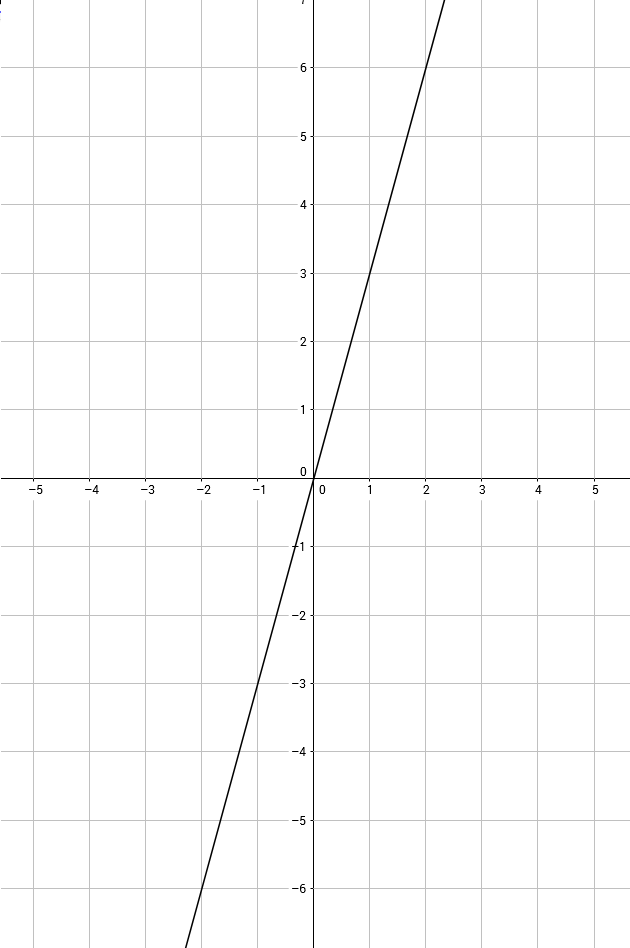
\includegraphics[scale = 0.5]{figures/3X.png}
    \end{subfigure}%%
    \begin{subfigure}{.5\textwidth}
    \centering
    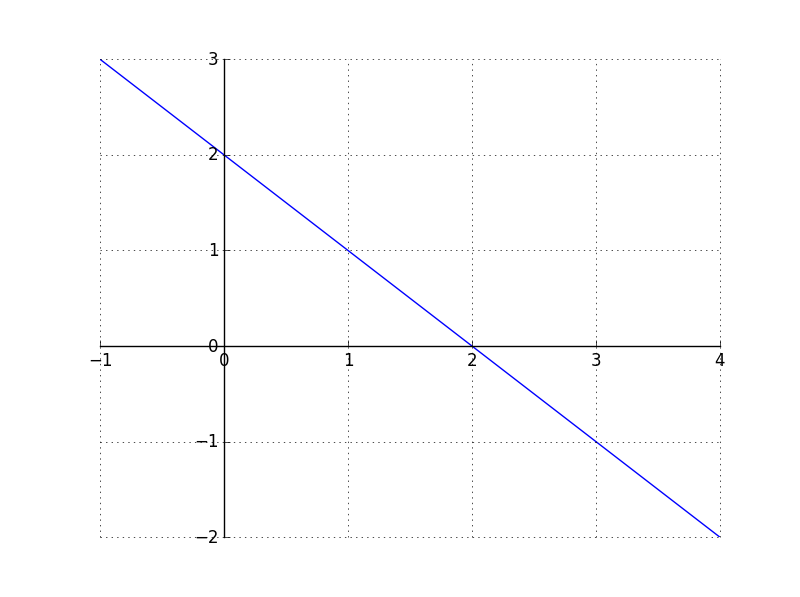
\includegraphics[scale = 0.5]{figures/mXp2.png}
    \end{subfigure}
    \begin{subfigure}{.5\textwidth}
    \centering
    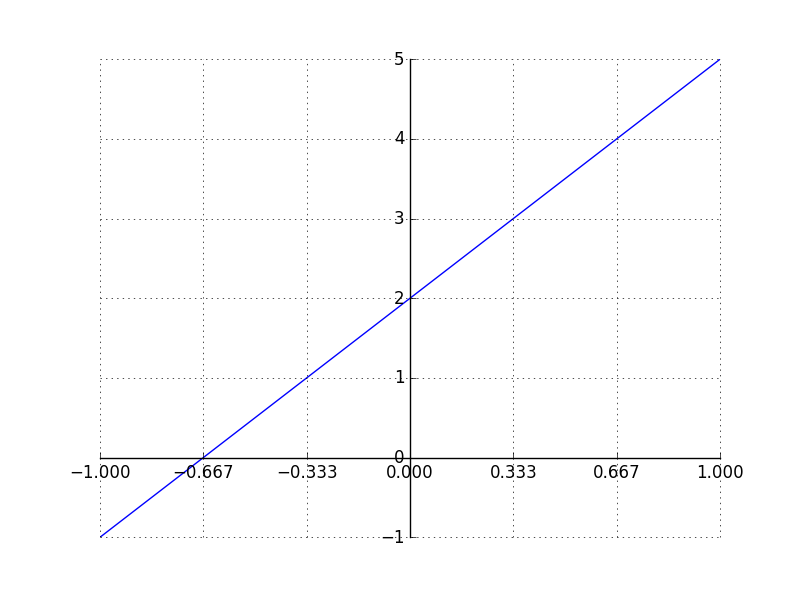
\includegraphics[scale = 0.5]{figures/3Xp2.png}
    \end{subfigure}%%
    \begin{subfigure}{.5\textwidth}
    \centering
    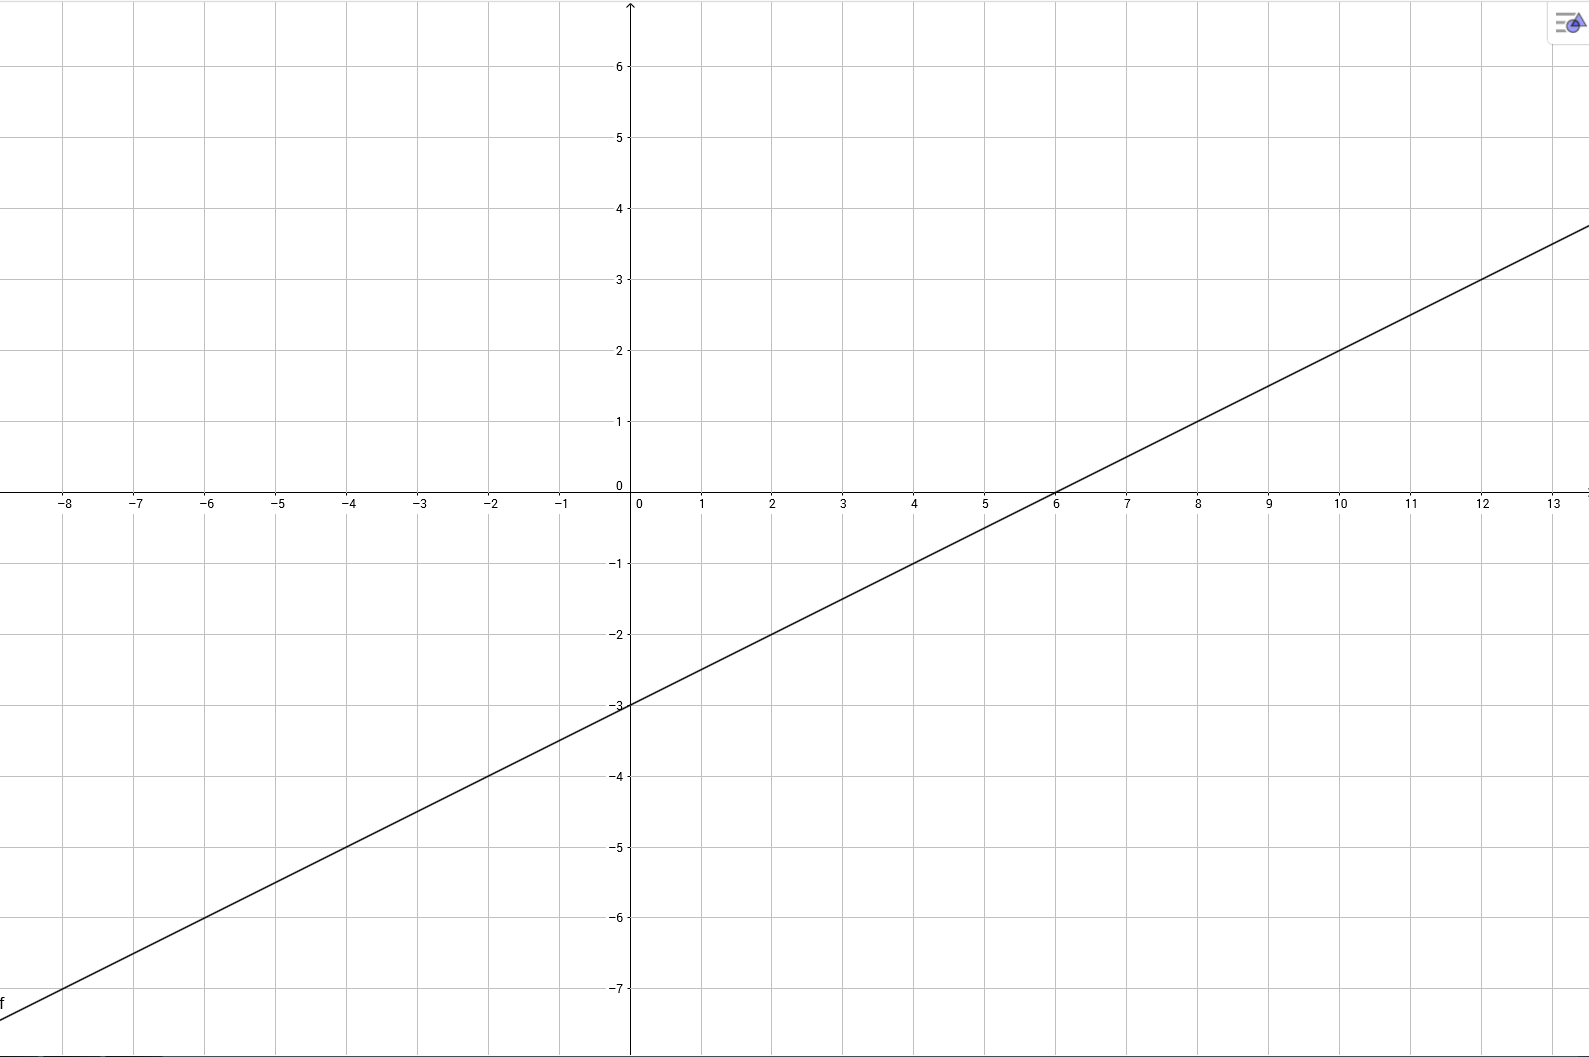
\includegraphics[scale = 0.5]{figures/05Xp2.png}
    \end{subfigure}
\end{figure}
{\color{Maroon}Hvis eleven forsatt ikke forstår vil da eleven presenteres med en video forklaring :  Video forklaring knappen dukker opp.}
\newline
\newline
\textbf{Video forklaring:}
\newline\newline
{\emph{\color{gray}
Husk at stigningstallet kan regnes ved å dele forandringen mellom y verdiene på forandringen i x-verdiene.}} 
\newline
{\color{PineGreen} På videoen vises formelen mens det forklares vha. grafen hvor oppleseren trekker en vertikal linje ned fra grafen fra en passelig funksonsverdi og deretter trekkes det en linje horisontalt inntil til funksjonen.} \newline\newline
{\emph{\color{gray}
Jeg kan velge passende $\Delta y$ og $\Delta x$ verdiene og sette disse inn i formelen for å regne ut stigningstallet.}} \newline
{\color{PineGreen} Det vises at oppleseren markerer $\Delta y$ og $\Delta x$ på grafen og skriver opp formelen.} 
\begin{figure}[h!]
\centering
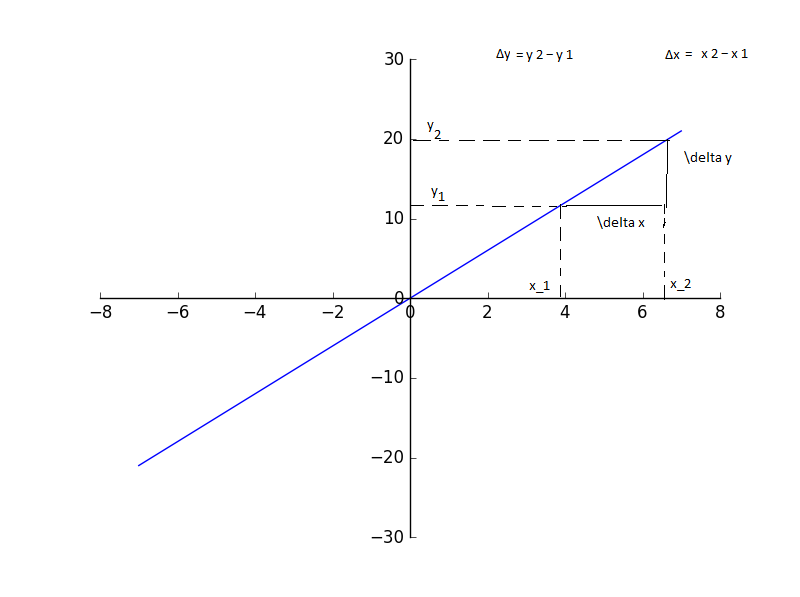
\includegraphics[scale = 0.6]{figures/stigningstallet.png}
\end{figure}
\newline\newline
{\emph{\color{gray}
F.eks i funksjonen $y = 3x$. Vi velger disse to punktene $y_2$ og $y_1$. Her ser vi at forandringen i y, er $\Delta y = y_2 - y_1 = 6- 0$ og forandringen i for disse funksjonsverdiene er $\Delta x_2 - \Delta x_1 = 2 - 0$. Da ser vi at stigningstallet blir $6/2 = 3.$}} \newline
{\color{PineGreen} Det vises at oppleseren gjentar avlesning fra funksjonen og markerer verdiene med striplet linje. Deretter setter oppleseren verdiene inn i formelen og regner ut stigningstallet.}
\begin{figure}[h!]
\centering
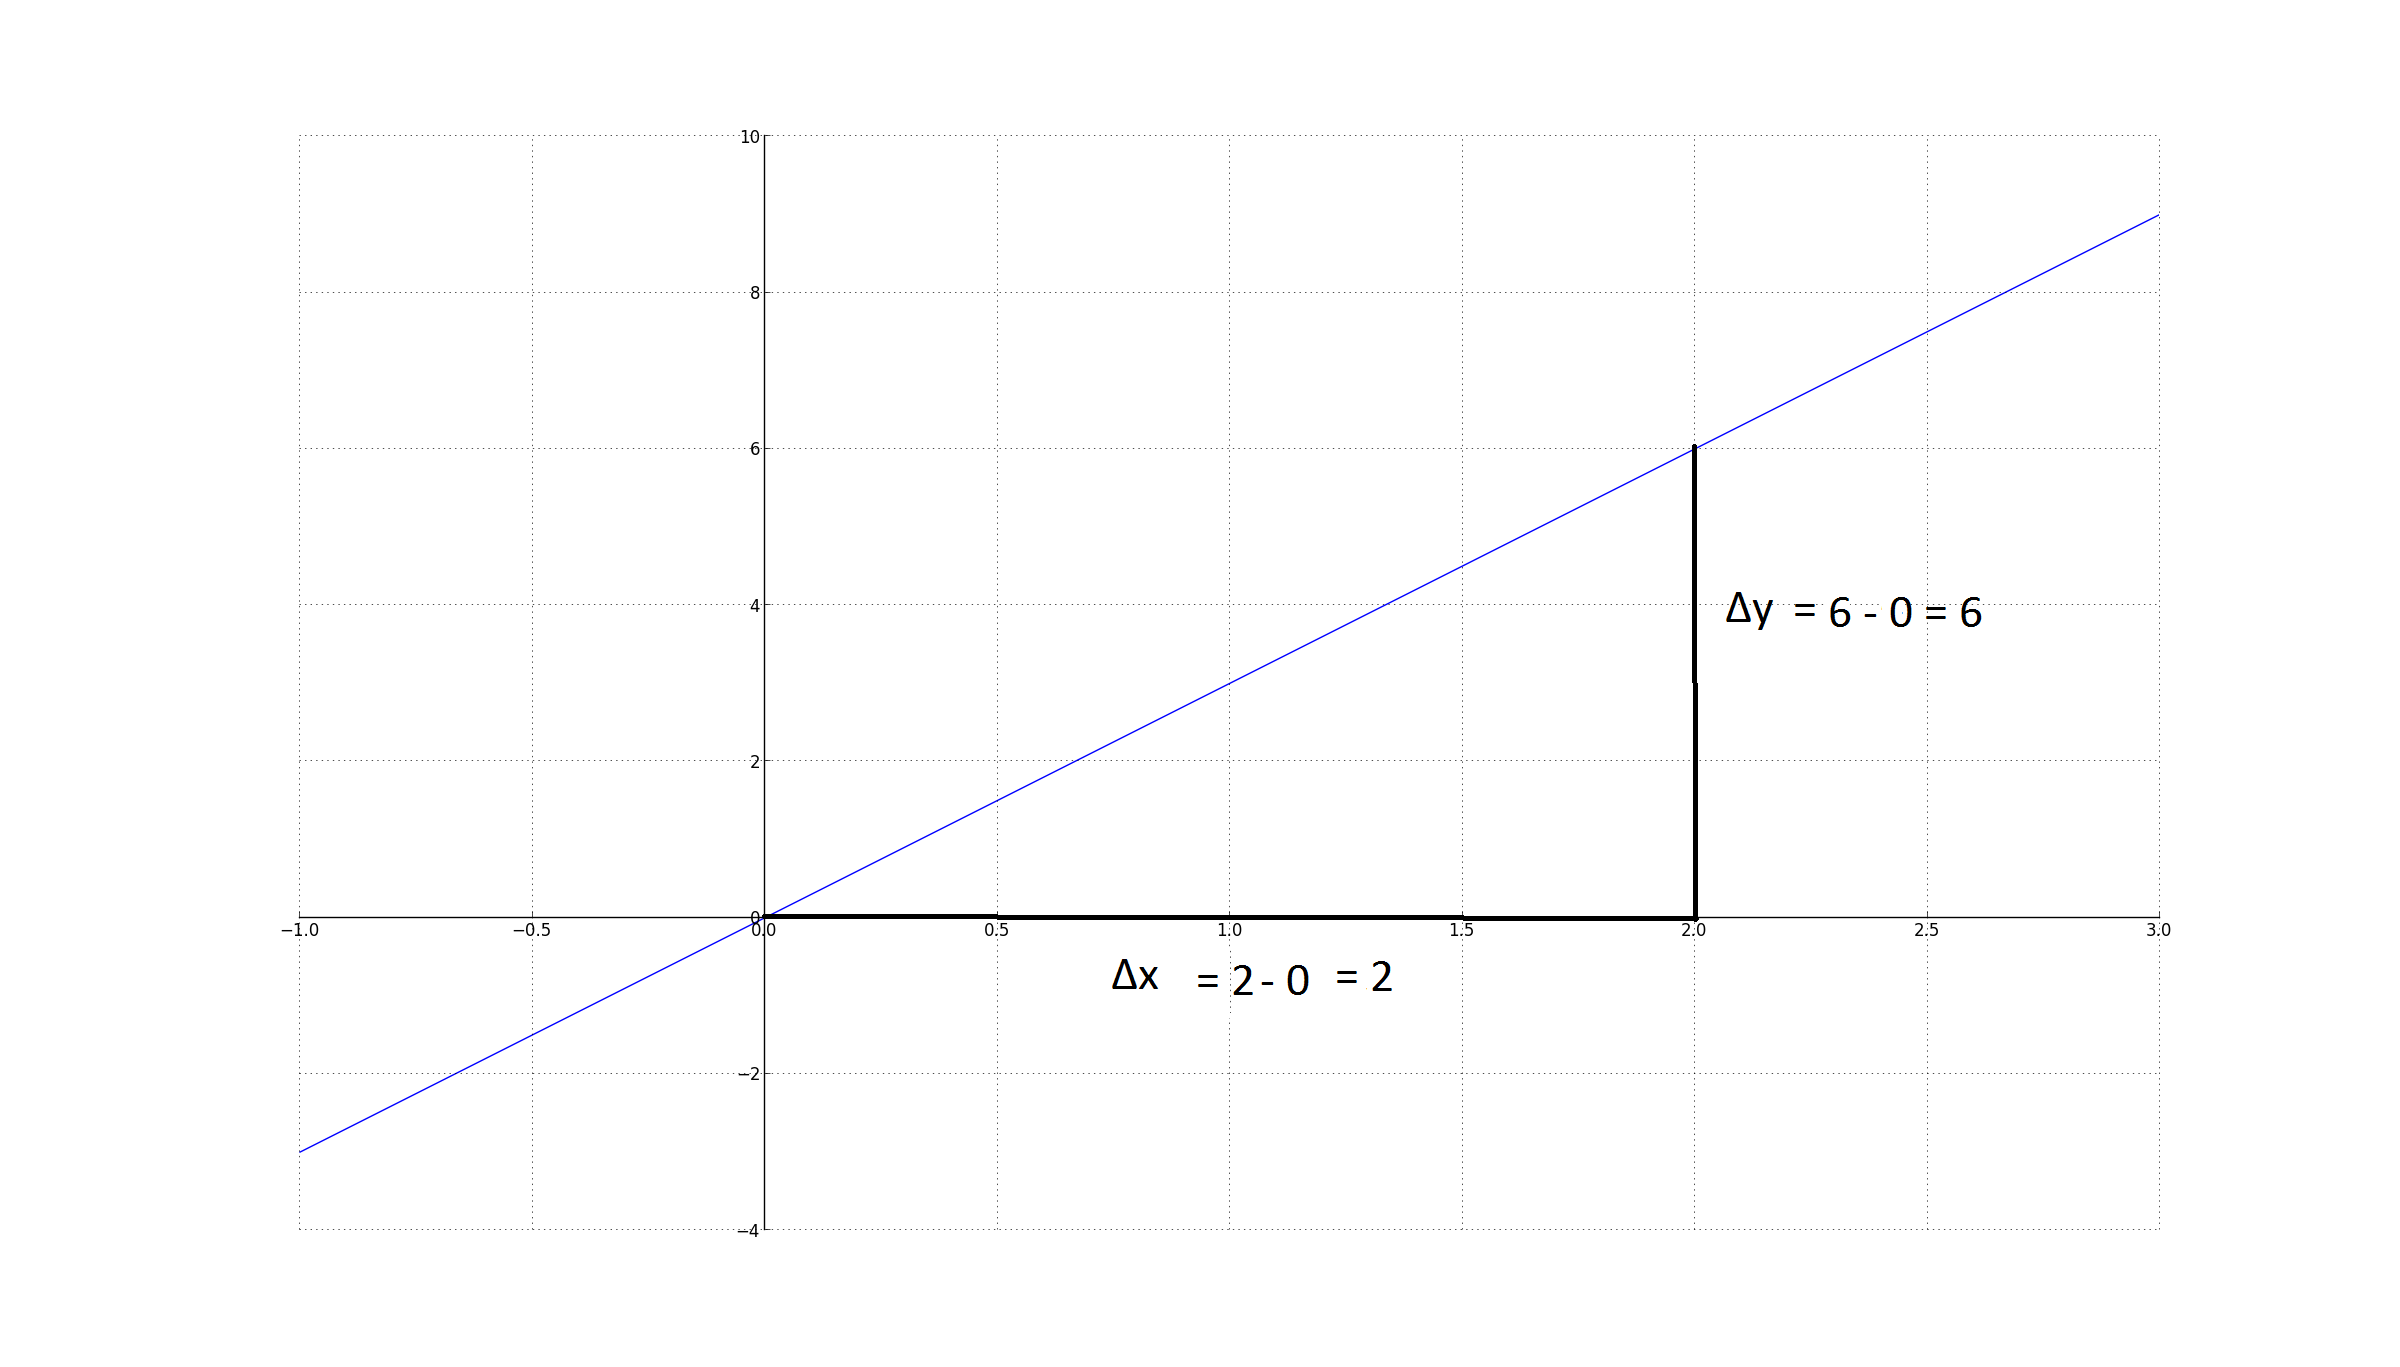
\includegraphics[scale = 0.3]{figures/stigningstalleksempelet.png}
\end{figure}
\end{Exercise}

\newpage
\newpage
\newpage
\subsection*{Konstantledd}

\begin{Exercise}
Finn verdien til y hvor funksjonen krysser y-aksen. (Tast verdien i svarfeltet) {\color{Cerulean} Hvordan bør svarfeltet brukes. Her skal svaret være en tall og da føler vi at det vanlige svarfeltet (se figuren under) blir for pregende.}
\begin{figure}[h!]
\centering
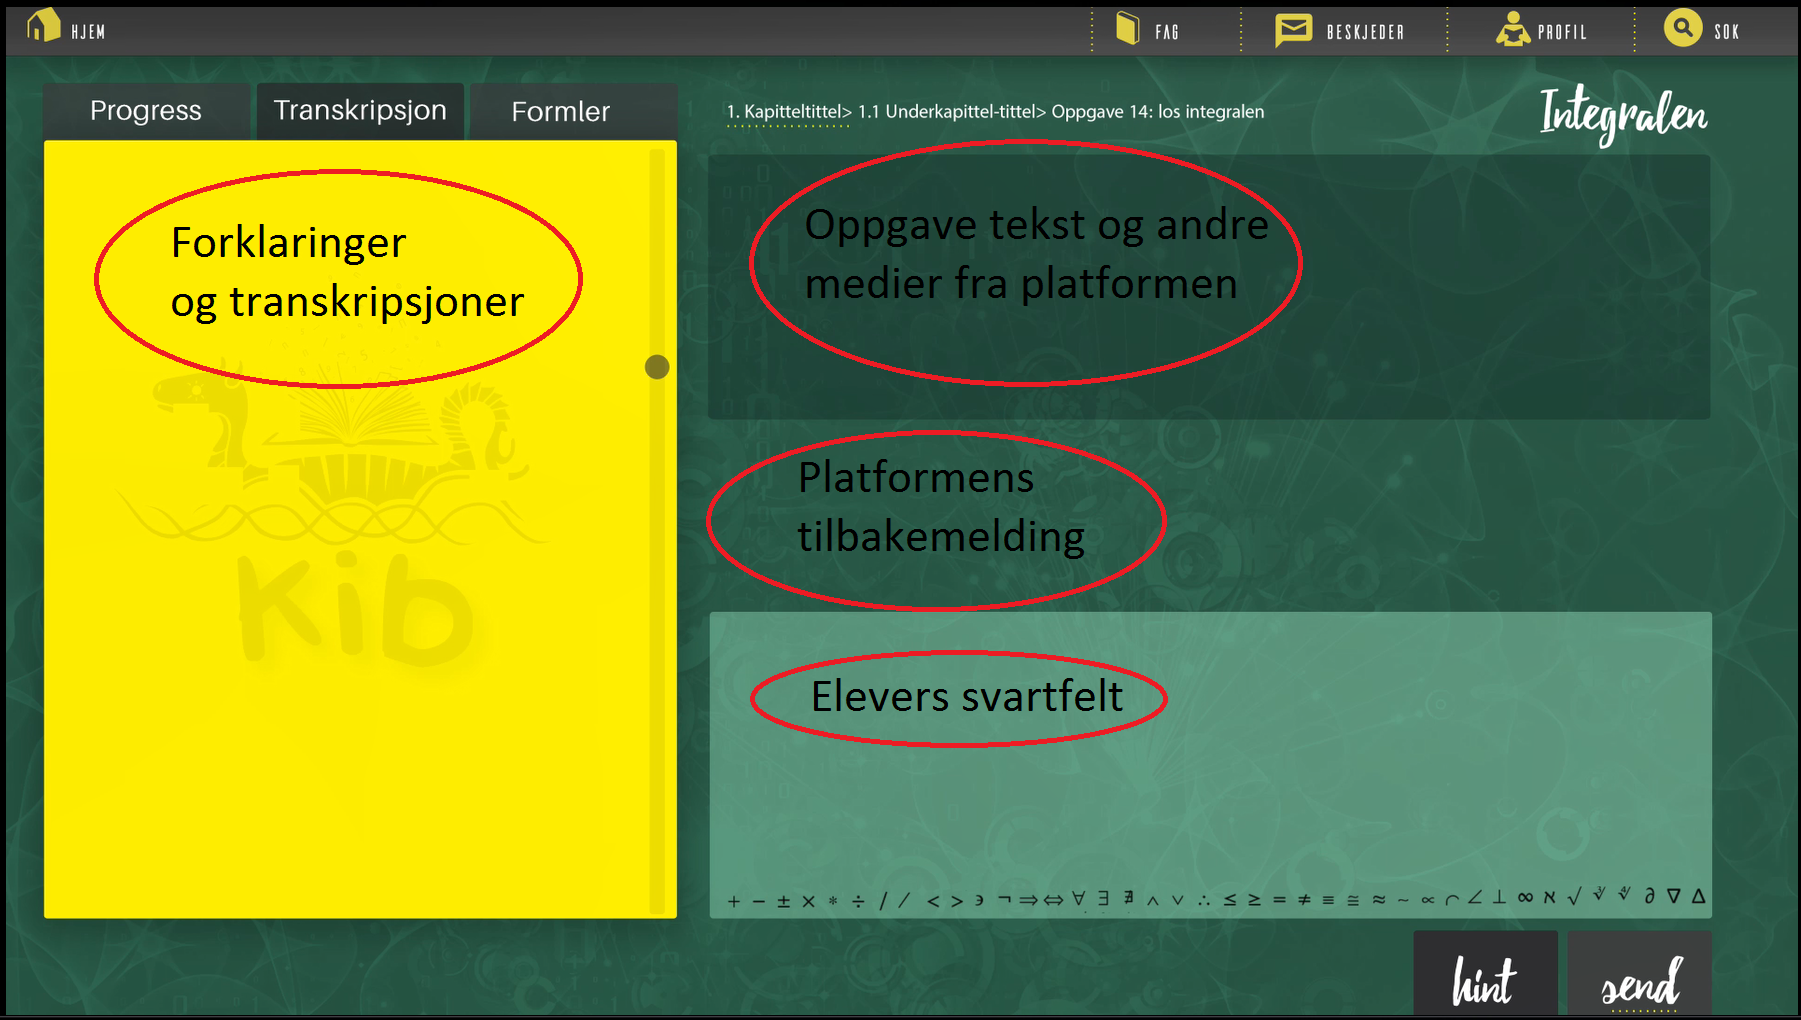
\includegraphics[scale = 0.3]{figures/Platform_explained.png}
\end{figure}
\end{Exercise}

\newpage
\begin{Exercise}
Finn konstantleddet til følgende lineære funksjoner. Fyll svaret i svarfeltet:
\begin{figure}[h!]
\centering
    \begin{subfigure}{.5\textwidth}
    \centering
    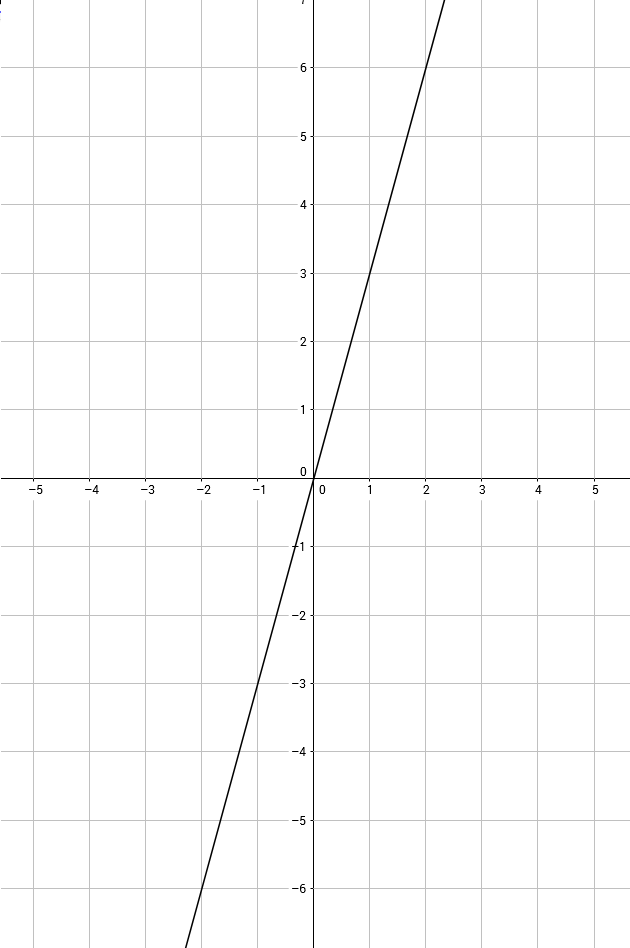
\includegraphics[scale = 0.5]{figures/3X.png}
    \end{subfigure}%%
    \begin{subfigure}{.5\textwidth}
    \centering
    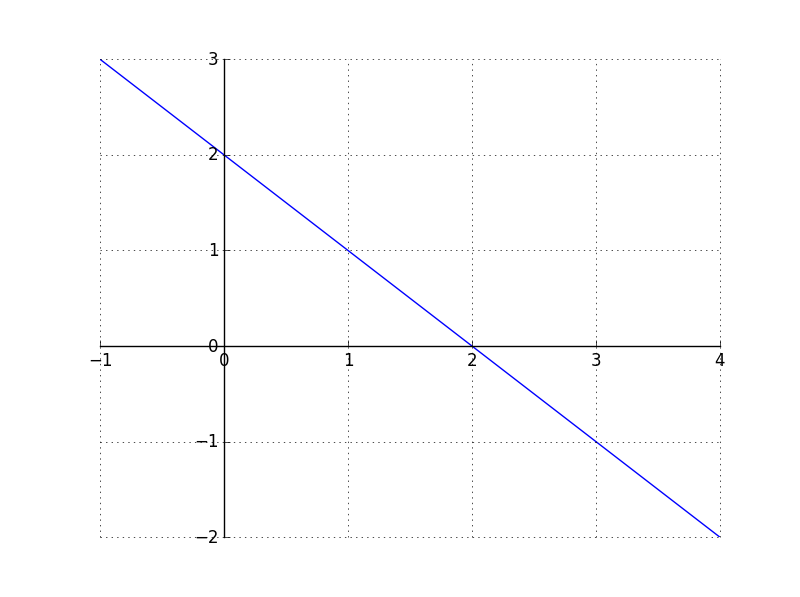
\includegraphics[scale = 0.5]{figures/mXp2.png}
    \end{subfigure}
    \begin{subfigure}{.5\textwidth}
    \centering
    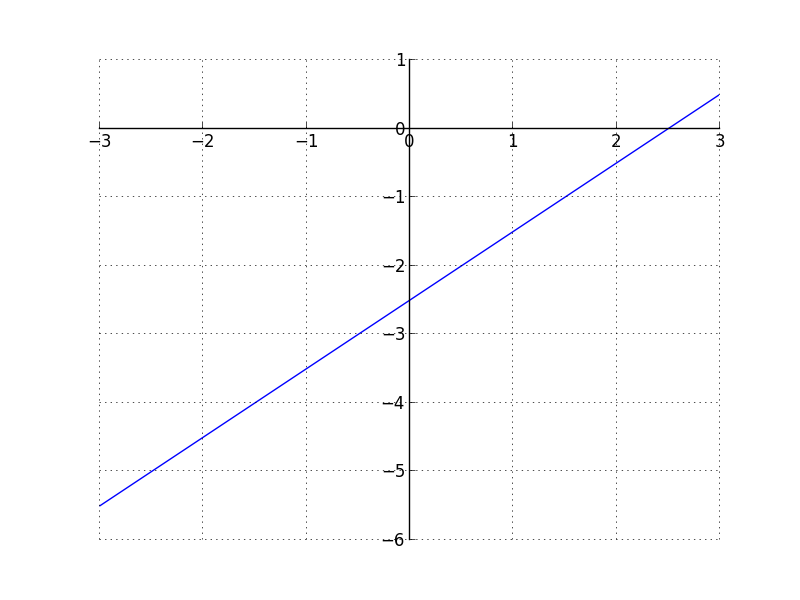
\includegraphics[scale = 0.5]{figures/Xm25.png}
    \end{subfigure}%%
    \begin{subfigure}{.5\textwidth}
    \centering
    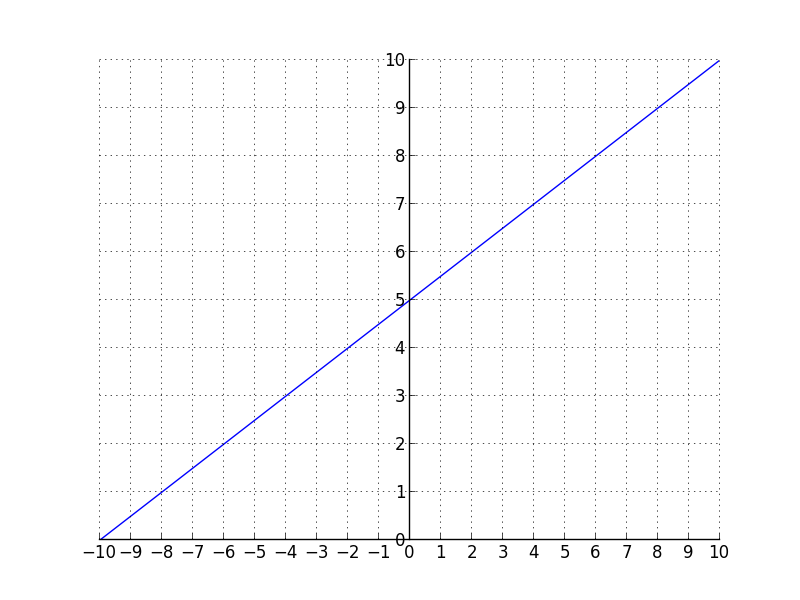
\includegraphics[scale = 0.5]{figures/05Xp5.png}
    \end{subfigure}
\end{figure}

{\color{Maroon}Hvis eleven taster feil:} \newline
{\color{gray}Husk at konstantleddet til funksjonen kan leses av figuren. Det er verdien til y der funksjonen krysser y-aksen.}
{\color{Maroon}Figur med utpekt verdi på funksjonen blir mens oppleseren forklarer eller tegner.}
\begin{figure}[h!]
\centering
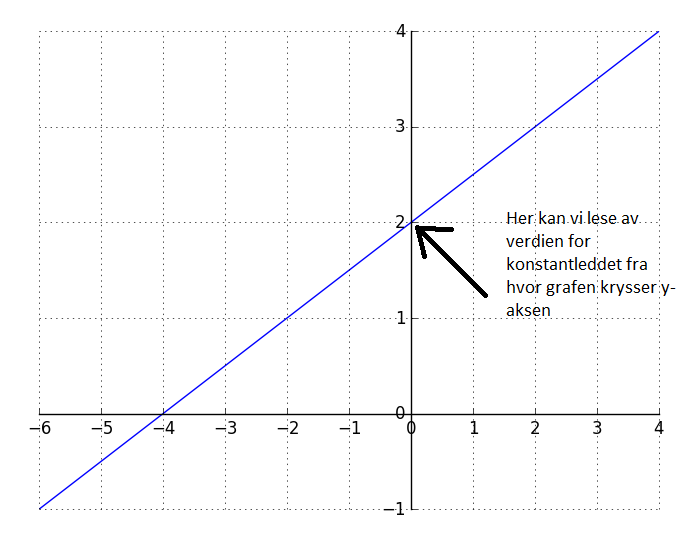
\includegraphics[scale = 0.4]{figures/konstantleddeksempelet.png}
\end{figure}
\end{Exercise}

\subsection*{Lineær funksjon}
I disse oppgavene  skal vi finne likninger til lineære funksjoner. Husk at en linje beskrives med likningen i formen $\mathbf{y} = {\color{blue}a}\mathbf{x}+ {\color{red}b}$ der ${\color{blue}a}$ er {\color{blue}stigningstallet} og ${\color{red}b}$ er \textbf{y} verdien ved krysnings punkt, dvs. {\color{red}konstantleddet}.

\begin{Exercise}
\textbf{Del 1)}
\newline
Skriv likning til linja som har stigningstallet $4$ og konstantledd $1$
\newline
\textbf{Svar}
\newline  
$y=4x+1$
\newline
\textbf{Hint 1}
\newline
Husk at likningen til en linje har formen $\mathbf{y} = {\color{blue}a}\mathbf{x}+ {\color{red}b}$ der ${\color{blue}a}$ er {\color{blue}stigningstallet} og ${\color{red}b}$ er {\color{red}konstantleddet}.
\newline
\textbf{Hint 2}
\newline
I dette tilfellet $a=4$ og $b=1$
\newline\newline
\textbf{Del 2)} 
\newline\newline
Hvilken graf tilhører denne funksjonen? 
\newline
{\color{Maroon}Det skal vises følgende funksjoner:
\newline
$y=4x+1$
\newline
$y=4x+5$
\newline
$y=1x+4$
\newline
$y=5x+3$
}
\begin{figure}[h!]
\centering
    \begin{subfigure}{.5\textwidth}
    \centering
    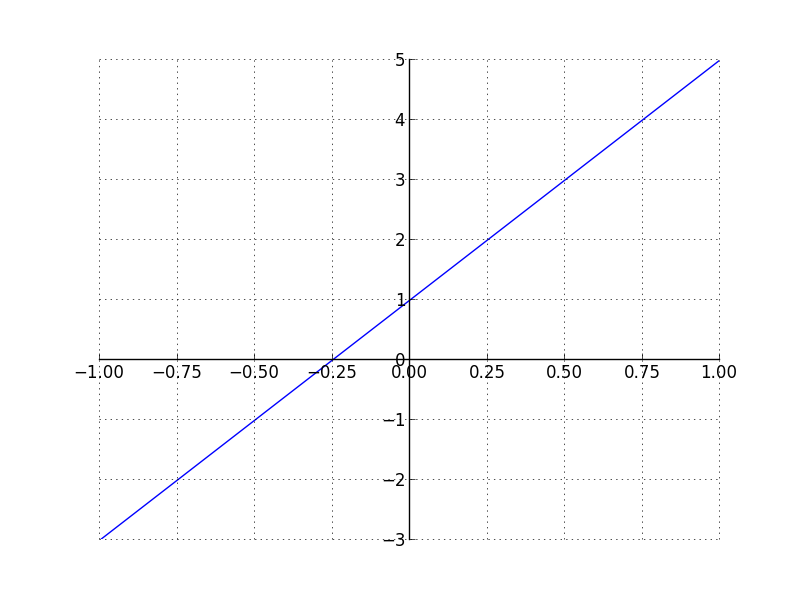
\includegraphics[scale = 0.5]{figures/4Xp1.png}
    \end{subfigure}%%
    \begin{subfigure}{.5\textwidth}
    \centering
    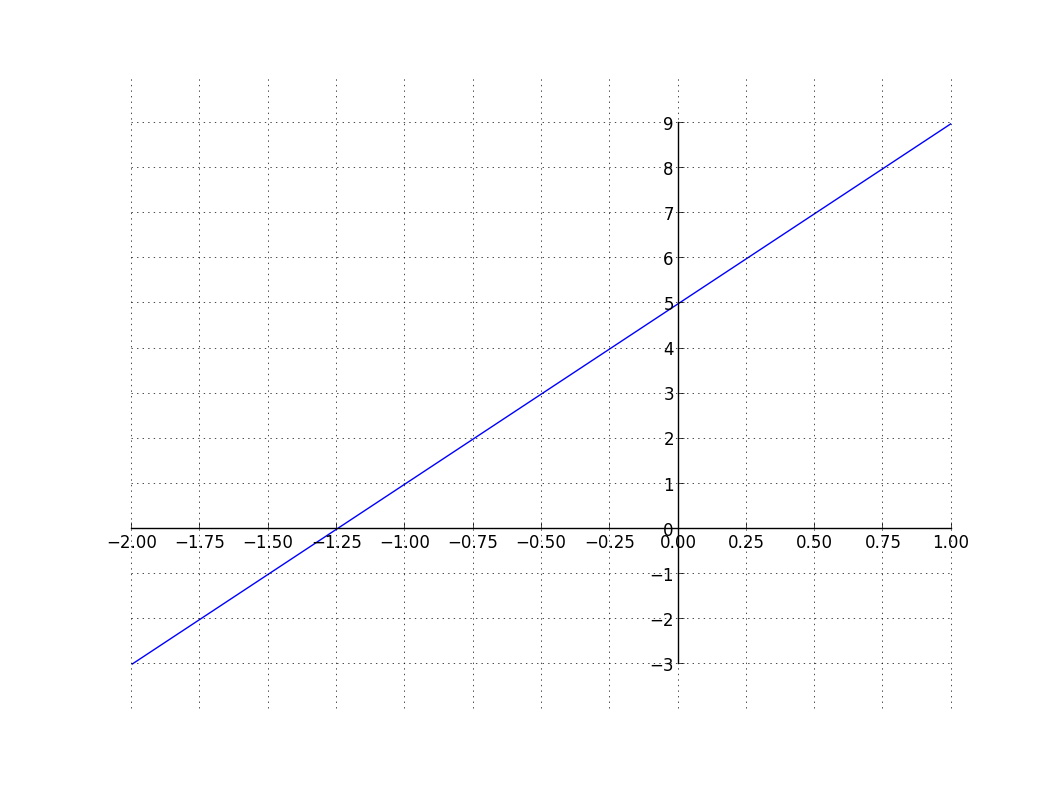
\includegraphics[scale = 0.4]{figures/4Xp5.png}
    \end{subfigure}
    \begin{subfigure}{.5\textwidth}
    \centering
    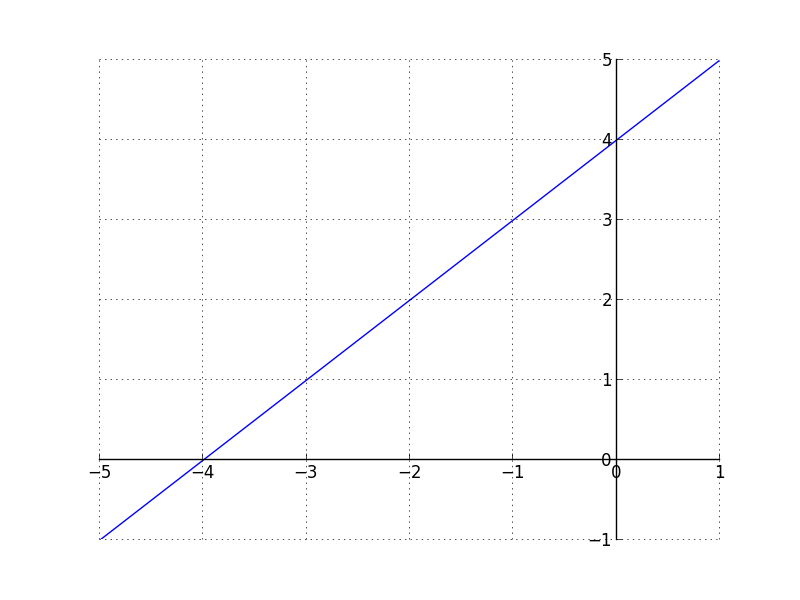
\includegraphics[scale = 0.5]{figures/Xp4.png}
    \end{subfigure}%%
    \begin{subfigure}{.5\textwidth}
    \centering
    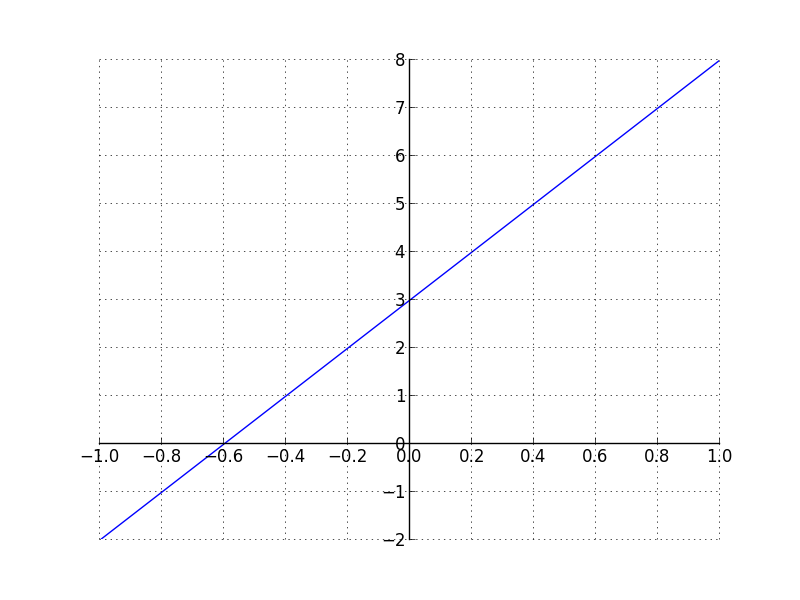
\includegraphics[scale = 0.5]{figures/5Xp3.png}
    \end{subfigure}
\end{figure}
\end{Exercise}

\begin{Exercise}
Skriv likning til linja som har stigningstallet $-2$ og som krysser y aksen på $3$
\newline\newline
\textbf{svar}  
\newline
$y=4x+1$
\newline
\textbf{Hint 1}
\newline
Husk at likningen til en linje har formen $y=ax+b$ der $a$ er stigningstallet og $b$ er y verdien ved krysnings punkt.
\newline
\textbf{Hint 2}
\newline
I dette tilfellet $a=-2$ og $b=3$
\newline\newline
\textbf{Oppgave 1.b} Hvilken graf tilhører denne funksjon? 
\newline
{\color{Maroon}Det skal vises følgende funksjoner:
\newline
$y=-2x+3$
\newline
$y=2x+-3$
\newline
$y=-3x+2$
\newline
$y=-3x+3$
}
\end{Exercise}

\begin{Exercise}
Skriv likningen som beskriver linear funksjon som vises i denne grafen:
\newline
{\color{Maroon} The graph will show this linear function: $y = 6x-3$:}
\newline
\newline
\textbf{Hint 1}
\newline
Husk at likningen til en linje har formen $y=ax+b$ der $a$ er stigningstallet og $b$ er y verdien ved krysnings punkt.
Hva er stigningstallet til denne linearfunskjon? 
$a=$
Hvor krysser funksjonen y aksen? 
$b=$
\end{Exercise}

\begin{Exercise}
Finn likning til linja som går gjenomm punktene $(2,6)$  og  $(0,-4 )$
\newline\newline
\textbf{Hint :}\newline 
Likning til en linje er på denne formen:
\begin{align}
y=\mathbf{a}x+ \mathbf{b}
\end{align}
Det vil si at vi vil finne stigninstallet $\mathbf{a}$ og konstantleddet $\mathbf{b}$.
\newline\newline
{\color{Maroon}Hvis elev forsatt sitter fast gis det et løsningsforslag -  for denne oppgavene der løsningen gitt gjennom skritt for skritt veiledning. Det antas heretter at eleven har svak forståelse}

\begin{enumerate}
\item Først kan vi finne stigninstallet $\mathbf{a}$  ved å bruke formelen:

{\color{white}
\begin{align}
a =  \frac{y_2 - y_1}{x_2 - x_1}
\end{align}
}
med de gitte punktene
$
\begin{matrix}
  x_1\:\:\: y_1 \\ 
 (0,\:-4) \\
\phantom{0}
\end{matrix}
$ og $
\begin{matrix}
  x_2\:\:\: y_2 \\ 
 (2,\:\:\:6)  \\
\phantom{0}
\end{matrix}
$ 

{\color{Maroon} Det oppstår $a=\frac{\:\:\:\:*\:\:\:\:}{\:\:\:\:*\:\:\:\:}$ på svarefeltet.
Hvis brukeren klarer ikke å fylle riktig tall selv, oppstår det en forklarings video}
\newline
\newline
{\color{gray}\emph{Pek og sett inn tallene i formelen.} }

{\color{Maroon}  Etter videoen må brukeren selv sette inn tallene.}

\item Sett inn verdien vi har funnet for stigningstallet i den opprinelige likgningen: $y = ax + b$
{\color{Maroon}
Hvis brukeren klarer ikke å fylle riktig tall selv, oppstår det formel i svarfeltet med blanktegn mens video forklarer hva bruker skal gjøre: 
\begin{align}
y = \underline{\phantom{0}}x + b
\end{align}}
{\color{gray}Sett in stigningstallet vi fant isted i formelen i svarfeltet. }

\item For å finne konstantleddet b, velger vi et punkt og ersatter koordinatene i ligningen og deretter løser vi ligningen for b. Sett opp ligningen og løs uttrykket.
{\color{Maroon} Hvis bruker klarer ikke å sette opp en ligning for b, får han veiledning til å sette opp ligningen. Bruker trykker på hjelpeknappen}
{\color{gray}\emph{Video viser forklaring med punktet (2,6) og deretter løser eleven punktet (0,-4) selv.} }
\begin{align}
(\:) = 5\cdot(\:) + b\\
(\, -4 \, ) = 5\cdot (\, 0 \, ) + b \\
b = -4
\end{align}

\item Siste skritt for å svare på oppgaven er å skrive opp utrrykket for funksjonen ved hjelp av stigningstallet a og konstantleddet b.
{\color{Maroon}
Hvis brukerer vet ikke hva han skal gjøre får han \mbox{hintent :}} \newline
\textbf{Hint:} husk at ligningen for funksjonen er gitt ved 
\begin{align}
y = ax + b
\end{align}
{\color{Maroon}
Hvis brukerer forsatt vet ikke hva han skal gjøre :}
\begin{align}
y = (\:)x + (\:)\\
y = (\, 5 \, )x  + (-4 )  \\
y = 5x - 4
\end{align}
\end{enumerate}

{\color{Maroon}Tilslutt skal det gis følgende oppsummering :}
\begin{itemize}
\item Finn først stigningstallet ved å bruke formelen :
\begin{align}
a =  \frac{y_2 - y_1}{x_2 - x_1}
\end{align}
\item Sett inn stigningstalllet i funksjonen og løs ligning for konstantleddet b:
\begin{itemize}
\item Sett opp et uttrykk for ligningen hvor b er ukjent :
\begin{align}
b = y_1 - a\cdot x_1
\end{align}
\item Velg et punkt $(x_1, y_1)$ og sett den inn for uttrykket for b
\end{itemize}
\end{itemize}
\end{Exercise}

\end{document}
